\chapter{Baseline}
\label{ch:baseline}

Before we can start analyzing any data or to do any algorithm research, we need to clarify what exact data we want to process and what results we want to gather. In this chapter we explain the preprocessing of the data from the collection from the Google server over normalization up to the clean up. Then we craft a precise description of the what we think similarity is in our context. Finally we present prior work on how to calculate this and explain why these methods do not work in our case.



\section{Data}
\label{sec:baseline:data}

\begin{figure}
    \centering
    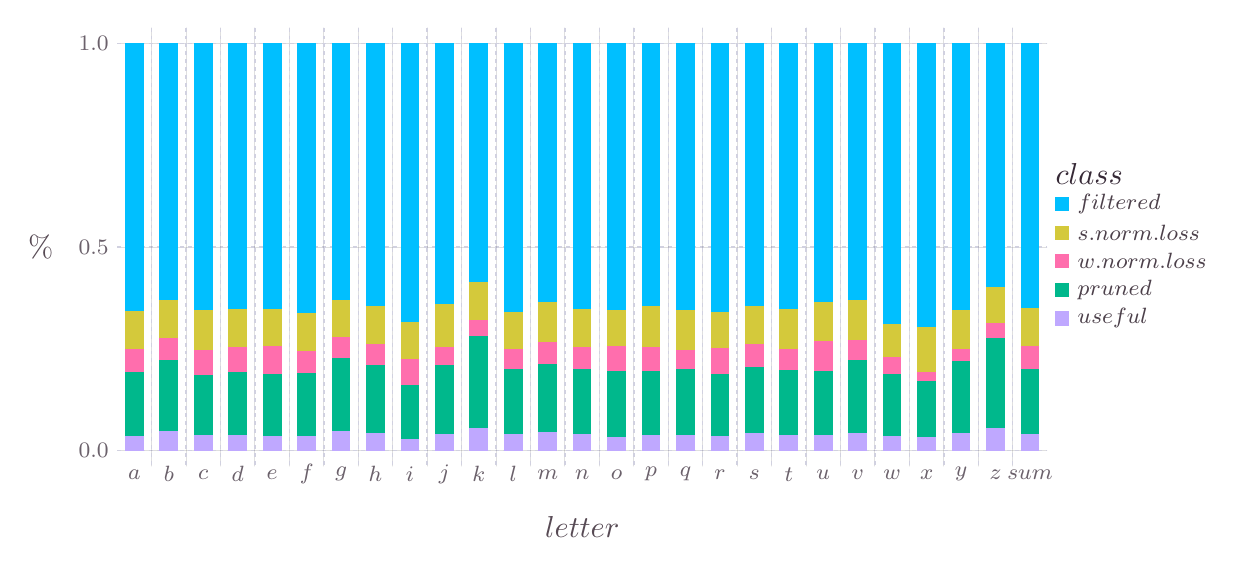
\begin{tikzpicture}[x=1mm,y=-1mm]
\definecolor{mycolorD4CA3A}{rgb}{0.83,0.79,0.23}
\definecolor{mycolor4C404B}{rgb}{0.3,0.25,0.29}
\definecolor{mycolor00BFFF}{rgb}{0,0.75,1}
\definecolor{mycolorD0D0E0}{rgb}{0.82,0.82,0.88}
\definecolor{mycolor362A35}{rgb}{0.21,0.16,0.21}
\definecolor{mycolor000000}{rgb}{0,0,0}
\definecolor{mycolor000000}{rgb}{0,0,0}
\definecolor{mycolor00B78D}{rgb}{0,0.72,0.55}
\definecolor{mycolor6C606B}{rgb}{0.42,0.38,0.42}
\definecolor{mycolorBEA9FF}{rgb}{0.75,0.66,1}
\definecolor{mycolorFF6DAE}{rgb}{1,0.43,0.68}
\definecolor{mycolor564A55}{rgb}{0.34,0.29,0.33}
\begin{scope}
\begin{scope}
\draw (77.07,68.39) node [text=mycolor564A55,draw=mycolor000000,draw opacity=0,rotate around={-0: (0,1.81)},inner sep=0.0]{\fontsize{3.88mm}{4.66mm}\selectfont $\text{letter}$};
\end{scope}
\begin{scope}
\draw (20.2,61.72) node [text=mycolor6C606B,rotate around={-0: (56.87,1.34)},inner sep=0.0]{\fontsize{2.82mm}{3.39mm}\selectfont $\text{a}$};
\draw (24.58,61.72) node [text=mycolor6C606B,rotate around={-0: (52.49,1.34)},inner sep=0.0]{\fontsize{2.82mm}{3.39mm}\selectfont $\text{b}$};
\draw (28.95,61.72) node [text=mycolor6C606B,rotate around={-0: (48.12,1.34)},inner sep=0.0]{\fontsize{2.82mm}{3.39mm}\selectfont $\text{c}$};
\draw (33.33,61.72) node [text=mycolor6C606B,rotate around={-0: (43.74,1.34)},inner sep=0.0]{\fontsize{2.82mm}{3.39mm}\selectfont $\text{d}$};
\draw (37.7,61.72) node [text=mycolor6C606B,rotate around={-0: (39.37,1.34)},inner sep=0.0]{\fontsize{2.82mm}{3.39mm}\selectfont $\text{e}$};
\draw (42.08,61.72) node [text=mycolor6C606B,rotate around={-0: (35,1.34)},inner sep=0.0]{\fontsize{2.82mm}{3.39mm}\selectfont $\text{f}$};
\draw (46.45,61.72) node [text=mycolor6C606B,rotate around={-0: (30.62,1.34)},inner sep=0.0]{\fontsize{2.82mm}{3.39mm}\selectfont $\text{g}$};
\draw (50.83,61.72) node [text=mycolor6C606B,rotate around={-0: (26.25,1.34)},inner sep=0.0]{\fontsize{2.82mm}{3.39mm}\selectfont $\text{h}$};
\draw (55.2,61.72) node [text=mycolor6C606B,rotate around={-0: (21.87,1.34)},inner sep=0.0]{\fontsize{2.82mm}{3.39mm}\selectfont $\text{i}$};
\draw (59.57,61.72) node [text=mycolor6C606B,rotate around={-0: (17.5,1.34)},inner sep=0.0]{\fontsize{2.82mm}{3.39mm}\selectfont $\text{j}$};
\draw (63.95,61.72) node [text=mycolor6C606B,rotate around={-0: (13.12,1.34)},inner sep=0.0]{\fontsize{2.82mm}{3.39mm}\selectfont $\text{k}$};
\draw (68.32,61.72) node [text=mycolor6C606B,rotate around={-0: (8.75,1.34)},inner sep=0.0]{\fontsize{2.82mm}{3.39mm}\selectfont $\text{l}$};
\draw (72.7,61.72) node [text=mycolor6C606B,rotate around={-0: (4.37,1.34)},inner sep=0.0]{\fontsize{2.82mm}{3.39mm}\selectfont $\text{m}$};
\draw (77.07,61.72) node [text=mycolor6C606B,rotate around={-0: (0,1.34)},inner sep=0.0]{\fontsize{2.82mm}{3.39mm}\selectfont $\text{n}$};
\draw (81.45,61.72) node [text=mycolor6C606B,rotate around={-0: (-4.37,1.34)},inner sep=0.0]{\fontsize{2.82mm}{3.39mm}\selectfont $\text{o}$};
\draw (85.82,61.72) node [text=mycolor6C606B,rotate around={-0: (-8.75,1.34)},inner sep=0.0]{\fontsize{2.82mm}{3.39mm}\selectfont $\text{p}$};
\draw (90.2,61.72) node [text=mycolor6C606B,rotate around={-0: (-13.12,1.34)},inner sep=0.0]{\fontsize{2.82mm}{3.39mm}\selectfont $\text{q}$};
\draw (94.57,61.72) node [text=mycolor6C606B,rotate around={-0: (-17.5,1.34)},inner sep=0.0]{\fontsize{2.82mm}{3.39mm}\selectfont $\text{r}$};
\draw (98.94,61.72) node [text=mycolor6C606B,rotate around={-0: (-21.87,1.34)},inner sep=0.0]{\fontsize{2.82mm}{3.39mm}\selectfont $\text{s}$};
\draw (103.32,61.72) node [text=mycolor6C606B,rotate around={-0: (-26.25,1.34)},inner sep=0.0]{\fontsize{2.82mm}{3.39mm}\selectfont $\text{t}$};
\draw (107.69,61.72) node [text=mycolor6C606B,rotate around={-0: (-30.62,1.34)},inner sep=0.0]{\fontsize{2.82mm}{3.39mm}\selectfont $\text{u}$};
\draw (112.07,61.72) node [text=mycolor6C606B,rotate around={-0: (-35,1.34)},inner sep=0.0]{\fontsize{2.82mm}{3.39mm}\selectfont $\text{v}$};
\draw (116.44,61.72) node [text=mycolor6C606B,rotate around={-0: (-39.37,1.34)},inner sep=0.0]{\fontsize{2.82mm}{3.39mm}\selectfont $\text{w}$};
\draw (120.82,61.72) node [text=mycolor6C606B,rotate around={-0: (-43.74,1.34)},inner sep=0.0]{\fontsize{2.82mm}{3.39mm}\selectfont $\text{x}$};
\draw (125.19,61.72) node [text=mycolor6C606B,rotate around={-0: (-48.12,1.34)},inner sep=0.0]{\fontsize{2.82mm}{3.39mm}\selectfont $\text{y}$};
\draw (129.57,61.72) node [text=mycolor6C606B,rotate around={-0: (-52.49,1.34)},inner sep=0.0]{\fontsize{2.82mm}{3.39mm}\selectfont $\text{z}$};
\draw (133.94,61.72) node [text=mycolor6C606B,rotate around={-0: (-56.87,1.34)},inner sep=0.0]{\fontsize{2.82mm}{3.39mm}\selectfont $\text{sum}$};
\end{scope}
\begin{scope}
\begin{scope}
\draw (139.94,27.42) node [text=mycolor4C404B,rotate around={-0: (5.62,5.44)},right,inner sep=0.0]{\fontsize{2.82mm}{3.39mm}\selectfont $\text{filtered}$};
\draw (139.94,31.04) node [text=mycolor4C404B,rotate around={-0: (5.62,1.81)},right,inner sep=0.0]{\fontsize{2.82mm}{3.39mm}\selectfont $\text{s.norm. loss}$};
\draw (139.94,34.67) node [text=mycolor4C404B,rotate around={-0: (5.62,-1.81)},right,inner sep=0.0]{\fontsize{2.82mm}{3.39mm}\selectfont $\text{w.norm. loss}$};
\draw (139.94,38.3) node [text=mycolor4C404B,rotate around={-0: (5.62,-5.44)},right,inner sep=0.0]{\fontsize{2.82mm}{3.39mm}\selectfont $\text{pruned}$};
\draw (139.94,41.92) node [text=mycolor4C404B,rotate around={-0: (5.62,-9.07)},right,inner sep=0.0]{\fontsize{2.82mm}{3.39mm}\selectfont $\text{useful}$};
\end{scope}
\begin{scope}
\path [fill=mycolor00BFFF,draw=mycolor000000,draw opacity=0] (137.13,26.51) rectangle +(1.81,1.81);
\path [fill=mycolorD4CA3A,draw=mycolor000000,draw opacity=0] (137.13,30.14) rectangle +(1.81,1.81);
\path [fill=mycolorFF6DAE,draw=mycolor000000,draw opacity=0] (137.13,33.76) rectangle +(1.81,1.81);
\path [fill=mycolor00B78D,draw=mycolor000000,draw opacity=0] (137.13,37.39) rectangle +(1.81,1.81);
\path [fill=mycolorBEA9FF,draw=mycolor000000,draw opacity=0] (137.13,41.02) rectangle +(1.81,1.81);
\end{scope}
\begin{scope}
\draw (137.13,23.6) node [text=mycolor362A35,draw=mycolor000000,draw opacity=0,rotate around={-0: (9.44,0.19)},right,inner sep=0.0]{\fontsize{3.88mm}{4.66mm}\selectfont $\text{class}$};
\end{scope}
\end{scope}
\begin{scope}
\clip  (18.02,5) -- (136.13,5) -- (136.13,60.72) -- (18.02,60.72);
\begin{scope}
\clip  (18.02,5) -- (136.13,5) -- (136.13,60.72) -- (18.02,60.72);
\path [fill=mycolor000000,fill opacity=0,draw=mycolor000000,draw opacity=0] (18.02,5) rectangle +(118.11,55.72);
\end{scope}
\begin{scope}
[dash pattern=on 0.5mm off 0.5mm,line width=0.2mm]
\path [fill=mycolor000000,draw=mycolorD0D0E0]  (18.02,58.72) -- (136.13,58.72);
\path [fill=mycolor000000,draw=mycolorD0D0E0]  (18.02,32.86) -- (136.13,32.86);
\path [fill=mycolor000000,draw=mycolorD0D0E0]  (18.02,7) -- (136.13,7);
\end{scope}
\begin{scope}
[dash pattern=on 0.5mm off 0.5mm,line width=0.2mm]
\path [fill=mycolor000000,draw=mycolorD0D0E0]  (22.39,5) -- (22.39,60.72);
\path [fill=mycolor000000,draw=mycolorD0D0E0]  (26.77,5) -- (26.77,60.72);
\path [fill=mycolor000000,draw=mycolorD0D0E0]  (31.14,5) -- (31.14,60.72);
\path [fill=mycolor000000,draw=mycolorD0D0E0]  (35.52,5) -- (35.52,60.72);
\path [fill=mycolor000000,draw=mycolorD0D0E0]  (39.89,5) -- (39.89,60.72);
\path [fill=mycolor000000,draw=mycolorD0D0E0]  (44.26,5) -- (44.26,60.72);
\path [fill=mycolor000000,draw=mycolorD0D0E0]  (48.64,5) -- (48.64,60.72);
\path [fill=mycolor000000,draw=mycolorD0D0E0]  (53.01,5) -- (53.01,60.72);
\path [fill=mycolor000000,draw=mycolorD0D0E0]  (57.39,5) -- (57.39,60.72);
\path [fill=mycolor000000,draw=mycolorD0D0E0]  (61.76,5) -- (61.76,60.72);
\path [fill=mycolor000000,draw=mycolorD0D0E0]  (66.14,5) -- (66.14,60.72);
\path [fill=mycolor000000,draw=mycolorD0D0E0]  (70.51,5) -- (70.51,60.72);
\path [fill=mycolor000000,draw=mycolorD0D0E0]  (74.88,5) -- (74.88,60.72);
\path [fill=mycolor000000,draw=mycolorD0D0E0]  (79.26,5) -- (79.26,60.72);
\path [fill=mycolor000000,draw=mycolorD0D0E0]  (83.63,5) -- (83.63,60.72);
\path [fill=mycolor000000,draw=mycolorD0D0E0]  (88.01,5) -- (88.01,60.72);
\path [fill=mycolor000000,draw=mycolorD0D0E0]  (92.38,5) -- (92.38,60.72);
\path [fill=mycolor000000,draw=mycolorD0D0E0]  (96.76,5) -- (96.76,60.72);
\path [fill=mycolor000000,draw=mycolorD0D0E0]  (101.13,5) -- (101.13,60.72);
\path [fill=mycolor000000,draw=mycolorD0D0E0]  (105.51,5) -- (105.51,60.72);
\path [fill=mycolor000000,draw=mycolorD0D0E0]  (109.88,5) -- (109.88,60.72);
\path [fill=mycolor000000,draw=mycolorD0D0E0]  (114.25,5) -- (114.25,60.72);
\path [fill=mycolor000000,draw=mycolorD0D0E0]  (118.63,5) -- (118.63,60.72);
\path [fill=mycolor000000,draw=mycolorD0D0E0]  (123,5) -- (123,60.72);
\path [fill=mycolor000000,draw=mycolorD0D0E0]  (127.38,5) -- (127.38,60.72);
\path [fill=mycolor000000,draw=mycolorD0D0E0]  (131.75,5) -- (131.75,60.72);
\end{scope}
\begin{scope}
\begin{scope}
[line width=0.3mm]
\begin{scope}
\path [fill=mycolorBEA9FF,draw=mycolor000000,draw opacity=0] (19.02,56.82) rectangle +(2.37,1.89);
\path [fill=mycolorBEA9FF,draw=mycolor000000,draw opacity=0] (23.39,56.26) rectangle +(2.37,2.46);
\path [fill=mycolorBEA9FF,draw=mycolor000000,draw opacity=0] (27.77,56.73) rectangle +(2.37,1.99);
\path [fill=mycolorBEA9FF,draw=mycolor000000,draw opacity=0] (32.14,56.7) rectangle +(2.37,2.01);
\path [fill=mycolorBEA9FF,draw=mycolor000000,draw opacity=0] (36.52,56.87) rectangle +(2.37,1.84);
\path [fill=mycolorBEA9FF,draw=mycolor000000,draw opacity=0] (40.89,56.81) rectangle +(2.37,1.9);
\path [fill=mycolorBEA9FF,draw=mycolor000000,draw opacity=0] (45.26,56.26) rectangle +(2.37,2.46);
\path [fill=mycolorBEA9FF,draw=mycolor000000,draw opacity=0] (49.64,56.46) rectangle +(2.37,2.26);
\path [fill=mycolorBEA9FF,draw=mycolor000000,draw opacity=0] (54.01,57.27) rectangle +(2.37,1.45);
\path [fill=mycolorBEA9FF,draw=mycolor000000,draw opacity=0] (58.39,56.61) rectangle +(2.37,2.1);
\path [fill=mycolorBEA9FF,draw=mycolor000000,draw opacity=0] (62.76,55.79) rectangle +(2.37,2.92);
\path [fill=mycolorBEA9FF,draw=mycolor000000,draw opacity=0] (67.14,56.62) rectangle +(2.37,2.09);
\path [fill=mycolorBEA9FF,draw=mycolor000000,draw opacity=0] (71.51,56.36) rectangle +(2.37,2.36);
\path [fill=mycolorBEA9FF,draw=mycolor000000,draw opacity=0] (75.88,56.56) rectangle +(2.37,2.16);
\path [fill=mycolorBEA9FF,draw=mycolor000000,draw opacity=0] (80.26,56.98) rectangle +(2.37,1.74);
\path [fill=mycolorBEA9FF,draw=mycolor000000,draw opacity=0] (84.63,56.69) rectangle +(2.37,2.03);
\path [fill=mycolorBEA9FF,draw=mycolor000000,draw opacity=0] (89.01,56.74) rectangle +(2.37,1.97);
\path [fill=mycolorBEA9FF,draw=mycolor000000,draw opacity=0] (93.38,56.8) rectangle +(2.37,1.91);
\path [fill=mycolorBEA9FF,draw=mycolor000000,draw opacity=0] (97.76,56.52) rectangle +(2.37,2.19);
\path [fill=mycolorBEA9FF,draw=mycolor000000,draw opacity=0] (102.13,56.73) rectangle +(2.37,1.98);
\path [fill=mycolorBEA9FF,draw=mycolor000000,draw opacity=0] (106.51,56.73) rectangle +(2.37,1.99);
\path [fill=mycolorBEA9FF,draw=mycolor000000,draw opacity=0] (110.88,56.52) rectangle +(2.37,2.19);
\path [fill=mycolorBEA9FF,draw=mycolor000000,draw opacity=0] (115.25,56.8) rectangle +(2.37,1.91);
\path [fill=mycolorBEA9FF,draw=mycolor000000,draw opacity=0] (119.63,56.98) rectangle +(2.37,1.74);
\path [fill=mycolorBEA9FF,draw=mycolor000000,draw opacity=0] (124,56.46) rectangle +(2.37,2.26);
\path [fill=mycolorBEA9FF,draw=mycolor000000,draw opacity=0] (128.38,55.85) rectangle +(2.37,2.86);
\path [fill=mycolorBEA9FF,draw=mycolor000000,draw opacity=0] (132.75,56.64) rectangle +(2.37,2.08);
\path [fill=mycolor00B78D,draw=mycolor000000,draw opacity=0] (19.02,48.78) rectangle +(2.37,8.04);
\path [fill=mycolor00B78D,draw=mycolor000000,draw opacity=0] (23.39,47.19) rectangle +(2.37,9.07);
\path [fill=mycolor00B78D,draw=mycolor000000,draw opacity=0] (27.77,49.08) rectangle +(2.37,7.65);
\path [fill=mycolor00B78D,draw=mycolor000000,draw opacity=0] (32.14,48.78) rectangle +(2.37,7.92);
\path [fill=mycolor00B78D,draw=mycolor000000,draw opacity=0] (36.52,49) rectangle +(2.37,7.87);
\path [fill=mycolor00B78D,draw=mycolor000000,draw opacity=0] (40.89,48.87) rectangle +(2.37,7.94);
\path [fill=mycolor00B78D,draw=mycolor000000,draw opacity=0] (45.26,47.01) rectangle +(2.37,9.24);
\path [fill=mycolor00B78D,draw=mycolor000000,draw opacity=0] (49.64,47.86) rectangle +(2.37,8.6);
\path [fill=mycolor00B78D,draw=mycolor000000,draw opacity=0] (54.01,50.39) rectangle +(2.37,6.88);
\path [fill=mycolor00B78D,draw=mycolor000000,draw opacity=0] (58.39,47.85) rectangle +(2.37,8.77);
\path [fill=mycolor00B78D,draw=mycolor000000,draw opacity=0] (62.76,44.21) rectangle +(2.37,11.58);
\path [fill=mycolor00B78D,draw=mycolor000000,draw opacity=0] (67.14,48.41) rectangle +(2.37,8.21);
\path [fill=mycolor00B78D,draw=mycolor000000,draw opacity=0] (71.51,47.73) rectangle +(2.37,8.63);
\path [fill=mycolor00B78D,draw=mycolor000000,draw opacity=0] (75.88,48.35) rectangle +(2.37,8.21);
\path [fill=mycolor00B78D,draw=mycolor000000,draw opacity=0] (80.26,48.64) rectangle +(2.37,8.34);
\path [fill=mycolor00B78D,draw=mycolor000000,draw opacity=0] (84.63,48.58) rectangle +(2.37,8.11);
\path [fill=mycolor00B78D,draw=mycolor000000,draw opacity=0] (89.01,48.33) rectangle +(2.37,8.41);
\path [fill=mycolor00B78D,draw=mycolor000000,draw opacity=0] (93.38,48.97) rectangle +(2.37,7.83);
\path [fill=mycolor00B78D,draw=mycolor000000,draw opacity=0] (97.76,48.04) rectangle +(2.37,8.48);
\path [fill=mycolor00B78D,draw=mycolor000000,draw opacity=0] (102.13,48.45) rectangle +(2.37,8.28);
\path [fill=mycolor00B78D,draw=mycolor000000,draw opacity=0] (106.51,48.64) rectangle +(2.37,8.09);
\path [fill=mycolor00B78D,draw=mycolor000000,draw opacity=0] (110.88,47.21) rectangle +(2.37,9.31);
\path [fill=mycolor00B78D,draw=mycolor000000,draw opacity=0] (115.25,48.95) rectangle +(2.37,7.86);
\path [fill=mycolor00B78D,draw=mycolor000000,draw opacity=0] (119.63,49.81) rectangle +(2.37,7.17);
\path [fill=mycolor00B78D,draw=mycolor000000,draw opacity=0] (124,47.36) rectangle +(2.37,9.1);
\path [fill=mycolor00B78D,draw=mycolor000000,draw opacity=0] (128.38,44.35) rectangle +(2.37,11.5);
\path [fill=mycolor00B78D,draw=mycolor000000,draw opacity=0] (132.75,48.31) rectangle +(2.37,8.33);
\path [fill=mycolorFF6DAE,draw=mycolor000000,draw opacity=0] (19.02,45.75) rectangle +(2.37,3.03);
\path [fill=mycolorFF6DAE,draw=mycolor000000,draw opacity=0] (23.39,44.4) rectangle +(2.37,2.79);
\path [fill=mycolorFF6DAE,draw=mycolor000000,draw opacity=0] (27.77,45.98) rectangle +(2.37,3.1);
\path [fill=mycolorFF6DAE,draw=mycolor000000,draw opacity=0] (32.14,45.55) rectangle +(2.37,3.23);
\path [fill=mycolorFF6DAE,draw=mycolor000000,draw opacity=0] (36.52,45.38) rectangle +(2.37,3.62);
\path [fill=mycolorFF6DAE,draw=mycolor000000,draw opacity=0] (40.89,46) rectangle +(2.37,2.87);
\path [fill=mycolorFF6DAE,draw=mycolor000000,draw opacity=0] (45.26,44.33) rectangle +(2.37,2.68);
\path [fill=mycolorFF6DAE,draw=mycolor000000,draw opacity=0] (49.64,45.21) rectangle +(2.37,2.64);
\path [fill=mycolorFF6DAE,draw=mycolor000000,draw opacity=0] (54.01,47.04) rectangle +(2.37,3.35);
\path [fill=mycolorFF6DAE,draw=mycolor000000,draw opacity=0] (58.39,45.57) rectangle +(2.37,2.28);
\path [fill=mycolorFF6DAE,draw=mycolor000000,draw opacity=0] (62.76,42.07) rectangle +(2.37,2.14);
\path [fill=mycolorFF6DAE,draw=mycolor000000,draw opacity=0] (67.14,45.85) rectangle +(2.37,2.56);
\path [fill=mycolorFF6DAE,draw=mycolor000000,draw opacity=0] (71.51,44.96) rectangle +(2.37,2.77);
\path [fill=mycolorFF6DAE,draw=mycolor000000,draw opacity=0] (75.88,45.56) rectangle +(2.37,2.78);
\path [fill=mycolorFF6DAE,draw=mycolor000000,draw opacity=0] (80.26,45.38) rectangle +(2.37,3.25);
\path [fill=mycolorFF6DAE,draw=mycolor000000,draw opacity=0] (84.63,45.51) rectangle +(2.37,3.07);
\path [fill=mycolorFF6DAE,draw=mycolor000000,draw opacity=0] (89.01,45.9) rectangle +(2.37,2.43);
\path [fill=mycolorFF6DAE,draw=mycolor000000,draw opacity=0] (93.38,45.65) rectangle +(2.37,3.32);
\path [fill=mycolorFF6DAE,draw=mycolor000000,draw opacity=0] (97.76,45.22) rectangle +(2.37,2.82);
\path [fill=mycolorFF6DAE,draw=mycolor000000,draw opacity=0] (102.13,45.83) rectangle +(2.37,2.63);
\path [fill=mycolorFF6DAE,draw=mycolor000000,draw opacity=0] (106.51,44.75) rectangle +(2.37,3.89);
\path [fill=mycolorFF6DAE,draw=mycolor000000,draw opacity=0] (110.88,44.63) rectangle +(2.37,2.58);
\path [fill=mycolorFF6DAE,draw=mycolor000000,draw opacity=0] (115.25,46.83) rectangle +(2.37,2.12);
\path [fill=mycolorFF6DAE,draw=mycolor000000,draw opacity=0] (119.63,48.69) rectangle +(2.37,1.12);
\path [fill=mycolorFF6DAE,draw=mycolor000000,draw opacity=0] (124,45.79) rectangle +(2.37,1.56);
\path [fill=mycolorFF6DAE,draw=mycolor000000,draw opacity=0] (128.38,42.47) rectangle +(2.37,1.88);
\path [fill=mycolorFF6DAE,draw=mycolor000000,draw opacity=0] (132.75,45.41) rectangle +(2.37,2.9);
\path [fill=mycolorD4CA3A,draw=mycolor000000,draw opacity=0] (19.02,40.99) rectangle +(2.37,4.76);
\path [fill=mycolorD4CA3A,draw=mycolor000000,draw opacity=0] (23.39,39.56) rectangle +(2.37,4.84);
\path [fill=mycolorD4CA3A,draw=mycolor000000,draw opacity=0] (27.77,40.91) rectangle +(2.37,5.07);
\path [fill=mycolorD4CA3A,draw=mycolor000000,draw opacity=0] (32.14,40.7) rectangle +(2.37,4.85);
\path [fill=mycolorD4CA3A,draw=mycolor000000,draw opacity=0] (36.52,40.71) rectangle +(2.37,4.68);
\path [fill=mycolorD4CA3A,draw=mycolor000000,draw opacity=0] (40.89,41.2) rectangle +(2.37,4.81);
\path [fill=mycolorD4CA3A,draw=mycolor000000,draw opacity=0] (45.26,39.54) rectangle +(2.37,4.79);
\path [fill=mycolorD4CA3A,draw=mycolor000000,draw opacity=0] (49.64,40.34) rectangle +(2.37,4.87);
\path [fill=mycolorD4CA3A,draw=mycolor000000,draw opacity=0] (54.01,42.33) rectangle +(2.37,4.71);
\path [fill=mycolorD4CA3A,draw=mycolor000000,draw opacity=0] (58.39,40.11) rectangle +(2.37,5.46);
\path [fill=mycolorD4CA3A,draw=mycolor000000,draw opacity=0] (62.76,37.27) rectangle +(2.37,4.8);
\path [fill=mycolorD4CA3A,draw=mycolor000000,draw opacity=0] (67.14,41.06) rectangle +(2.37,4.79);
\path [fill=mycolorD4CA3A,draw=mycolor000000,draw opacity=0] (71.51,39.88) rectangle +(2.37,5.08);
\path [fill=mycolorD4CA3A,draw=mycolor000000,draw opacity=0] (75.88,40.7) rectangle +(2.37,4.86);
\path [fill=mycolorD4CA3A,draw=mycolor000000,draw opacity=0] (80.26,40.81) rectangle +(2.37,4.57);
\path [fill=mycolorD4CA3A,draw=mycolor000000,draw opacity=0] (84.63,40.41) rectangle +(2.37,5.1);
\path [fill=mycolorD4CA3A,draw=mycolor000000,draw opacity=0] (89.01,40.88) rectangle +(2.37,5.02);
\path [fill=mycolorD4CA3A,draw=mycolor000000,draw opacity=0] (93.38,41.05) rectangle +(2.37,4.6);
\path [fill=mycolorD4CA3A,draw=mycolor000000,draw opacity=0] (97.76,40.3) rectangle +(2.37,4.92);
\path [fill=mycolorD4CA3A,draw=mycolor000000,draw opacity=0] (102.13,40.73) rectangle +(2.37,5.1);
\path [fill=mycolorD4CA3A,draw=mycolor000000,draw opacity=0] (106.51,39.82) rectangle +(2.37,4.92);
\path [fill=mycolorD4CA3A,draw=mycolor000000,draw opacity=0] (110.88,39.64) rectangle +(2.37,4.99);
\path [fill=mycolorD4CA3A,draw=mycolor000000,draw opacity=0] (115.25,42.61) rectangle +(2.37,4.22);
\path [fill=mycolorD4CA3A,draw=mycolor000000,draw opacity=0] (119.63,43) rectangle +(2.37,5.69);
\path [fill=mycolorD4CA3A,draw=mycolor000000,draw opacity=0] (124,40.89) rectangle +(2.37,4.9);
\path [fill=mycolorD4CA3A,draw=mycolor000000,draw opacity=0] (128.38,37.95) rectangle +(2.37,4.51);
\path [fill=mycolorD4CA3A,draw=mycolor000000,draw opacity=0] (132.75,40.54) rectangle +(2.37,4.87);
\path [fill=mycolor00BFFF,draw=mycolor000000,draw opacity=0] (19.02,7) rectangle +(2.37,33.99);
\path [fill=mycolor00BFFF,draw=mycolor000000,draw opacity=0] (23.39,7) rectangle +(2.37,32.56);
\path [fill=mycolor00BFFF,draw=mycolor000000,draw opacity=0] (27.77,7) rectangle +(2.37,33.91);
\path [fill=mycolor00BFFF,draw=mycolor000000,draw opacity=0] (32.14,7) rectangle +(2.37,33.7);
\path [fill=mycolor00BFFF,draw=mycolor000000,draw opacity=0] (36.52,7) rectangle +(2.37,33.71);
\path [fill=mycolor00BFFF,draw=mycolor000000,draw opacity=0] (40.89,7) rectangle +(2.37,34.2);
\path [fill=mycolor00BFFF,draw=mycolor000000,draw opacity=0] (45.26,7) rectangle +(2.37,32.54);
\path [fill=mycolor00BFFF,draw=mycolor000000,draw opacity=0] (49.64,7) rectangle +(2.37,33.34);
\path [fill=mycolor00BFFF,draw=mycolor000000,draw opacity=0] (54.01,7) rectangle +(2.37,35.33);
\path [fill=mycolor00BFFF,draw=mycolor000000,draw opacity=0] (58.39,7) rectangle +(2.37,33.11);
\path [fill=mycolor00BFFF,draw=mycolor000000,draw opacity=0] (62.76,7) rectangle +(2.37,30.27);
\path [fill=mycolor00BFFF,draw=mycolor000000,draw opacity=0] (67.14,7) rectangle +(2.37,34.06);
\path [fill=mycolor00BFFF,draw=mycolor000000,draw opacity=0] (71.51,7) rectangle +(2.37,32.88);
\path [fill=mycolor00BFFF,draw=mycolor000000,draw opacity=0] (75.88,7) rectangle +(2.37,33.7);
\path [fill=mycolor00BFFF,draw=mycolor000000,draw opacity=0] (80.26,7) rectangle +(2.37,33.81);
\path [fill=mycolor00BFFF,draw=mycolor000000,draw opacity=0] (84.63,7) rectangle +(2.37,33.41);
\path [fill=mycolor00BFFF,draw=mycolor000000,draw opacity=0] (89.01,7) rectangle +(2.37,33.88);
\path [fill=mycolor00BFFF,draw=mycolor000000,draw opacity=0] (93.38,7) rectangle +(2.37,34.05);
\path [fill=mycolor00BFFF,draw=mycolor000000,draw opacity=0] (97.76,7) rectangle +(2.37,33.3);
\path [fill=mycolor00BFFF,draw=mycolor000000,draw opacity=0] (102.13,7) rectangle +(2.37,33.73);
\path [fill=mycolor00BFFF,draw=mycolor000000,draw opacity=0] (106.51,7) rectangle +(2.37,32.82);
\path [fill=mycolor00BFFF,draw=mycolor000000,draw opacity=0] (110.88,7) rectangle +(2.37,32.64);
\path [fill=mycolor00BFFF,draw=mycolor000000,draw opacity=0] (115.25,7) rectangle +(2.37,35.61);
\path [fill=mycolor00BFFF,draw=mycolor000000,draw opacity=0] (119.63,7) rectangle +(2.37,36);
\path [fill=mycolor00BFFF,draw=mycolor000000,draw opacity=0] (124,7) rectangle +(2.37,33.89);
\path [fill=mycolor00BFFF,draw=mycolor000000,draw opacity=0] (128.38,7) rectangle +(2.37,30.95);
\path [fill=mycolor00BFFF,draw=mycolor000000,draw opacity=0] (132.75,7) rectangle +(2.37,33.54);
\end{scope}
\end{scope}
\end{scope}
\end{scope}
\begin{scope}
\draw (17.02,58.72) node [text=mycolor6C606B,rotate around={-0: (-2.01,-25.86)},left,inner sep=0.0]{\fontsize{2.82mm}{3.39mm}\selectfont $\text{0.0}$};
\draw (17.02,32.86) node [text=mycolor6C606B,rotate around={-0: (-2.01,-0)},left,inner sep=0.0]{\fontsize{2.82mm}{3.39mm}\selectfont $\text{0.5}$};
\draw (17.02,7) node [text=mycolor6C606B,rotate around={-0: (-2.01,25.86)},left,inner sep=0.0]{\fontsize{2.82mm}{3.39mm}\selectfont $\text{1.0}$};
\end{scope}
\begin{scope}
\draw (10,32.86) node [text=mycolor564A55,draw=mycolor000000,draw opacity=0,rotate around={-0: (-1.5,0)},left,inner sep=0.0]{\fontsize{3.88mm}{4.66mm}\selectfont $\text{\%}$};
\end{scope}
\end{scope}
\end{tikzpicture}

    \caption{Relative amount of pruned data per letter}\label{fig:clean_up_sums}
\end{figure}

We perform the following clean up steps:

\begin{enumerate}
    \itemsep0em
    \item download and parsing
    \item string filtering
    \item string normalization
    \item word normalization
    \item pruning
\end{enumerate}

Note that swapping the string-based steps does not lead a different output. \autoref{fig:clean_up_sums} show how much data is pruned by every step for the $1$-gram data set. The exact numbers can be found in \autoref{tab:clean_up_numbers_1} and \autoref{tab:clean_up_numbers_2}. Naturally there are some differences between the different starting characters but as far as we can tell no anomalies can be observed.


\subsection{Download and Parsing}
\label{ssec:baseline:data:download}
As a first step we download the raw data from the Google server. A complete list of download URLs can be obtained here:

\url{https://storage.googleapis.com/books/ngrams/books/datasetsv2.html}

The data collection and processing is described in~\cite{Google_nGrams}. The raw text data which was downloaded from the Google servers is mangled by a high-performance C++ implementation to speed-up the upcoming steps. During the first steps, only the nGram content is required without any knowledge of the actual time series data. We exploit this fact and delay the actual parsing and storage of the time series until the data is required and focus on the handling of the string data as long as possible.


\subsection{String filtering}
\label{ssec:baseline:data:filter}
It seems that the nGrams that Google extracted does not only contain pure words but also punctuation characters and word classes. To simplify storage of the strings and because our users are not interested in searching for whole word types, we filter out all entries that contain characters of the following class:

\code{\[_.,!'0-9\]}

\subsection{String Normalization}
\label{ssec:baseline:data:snorm}
Since the data the nGrams are described by Unicode strings, there may exist string describing the same content. We apply NFKC normalization as described in~\cite{unicode8annex15} to solve this issue. Furthermore we lowercase all inputs with respect to the Unicode standard. If this procedure will lead to duplicate nGrams, they are joined by adding the corresponding time series data.

Notice that the lowercase transformation may not work as expected for other languages than English since it may lead to a lose of important information.


\subsection{Word Normalization}
\label{ssec:baseline:data:wnorm}
The words forming the nGrams exist in multiple variants, e.g.\ different terms for verbs or singular and plural form for nouns. Naturally the resulting time series are very similar and do not contain valuable information, neither for our algorithms nor for a human analyst. We solve this issue by applying the WordNet lemmatizer (\cite{wordnet}) and afterwards the snowball stemmer (\cite{porter2}) to all words. In case of same output nGrams the related time series are added again.

As for the former transformation step be aware of the language problem. Other languages may require other word normalization techniques. Also there may be more advanced techniques that exploit the knowledge of the entire nGram instead of single words.

We decided not to run any OCR (optical character recognition) error recognition since we are not aware of any general purpose approach that does not transform rare words or names like a na\"{\i}ve spell checker would do.


\subsection{Pruning}
\label{ssec:baseline:data:prune}
The original data sets contains a lot of very rare nGrams that, in our opinion, do not provide enough statistical information to be considered during the further analysis. The same applies to all nGrams for the early years that are contained in the data. We decided to only use the last \num{256} years of the time series data and that we drop all nGrams where the related match count time series is too small, or in mathematical terms where $\sum_{1753 \leq y \leq 2008} v_{0, y} < 1000$ ($v_0$ is the \enquote{match count}) applies. Notice that this is the first step where the actual time series content is required. Therefore it is also the first step where we parse the time series data for all nGram strings which survived up to this point.

The selection of the time range of \num{256} years has other advantages apart from the pure pruning. Since it is a power of \num{2} it is easier to apply many transformations (e.g.\ Fourier or Discrete Wavelet Transformation) to it without the need to think about and justify additional edge case handling.



\section{Similarity}
\label{sec:baseline:sim}
We first discuss which time series we want to consider as similar. We want to explore which nGrams are used together. Because there might be a normal usage of certain words or phrases in the day to day life, interesting data might be hidden by an overall large number and therefore interesting changes in usage patterns might not be discovered when total numbers of mentions are compared. Consider the following example: $n_1 \Rightarrow n_2$ but not vice versa and $n_2$ is already used in many books but $n_1$ is a new nGram at a certain point of time. This implication cannot be found by comparing total numbers, because $n_2$ might be way larger than $n_1$ but the implication will lead to similar changes in the overall time series. So we seek to find similar structure instead of similar usage numbers.

\begin{definition}[Query]
    A query is a time series for which the user (or some program) wants to know the nearest neighbors for. By writing \enquote{some word} we refer to the time series which belongs to the normalized n-Gram or the n-Gram itself, depending on the context. The plural form queries is used to express multiple starting points for a nearest neighbor search, either when generating statistics or when calculating the distance to multiple time series.
\end{definition}

Furthermore we limit our analysis to the \enquote{match count} because it seems to be more useful for later research than the less fine grained \enquote{unique book count}.


\subsection{Normalization}
\label{ssec:baseline:sim:norm}

\begin{figure}
    \centering
    \begin{tikzpicture}
    \begin{axis}[
        xlabel={year},
        ylabel={$n$},
        x_year,
        legend pos=north west,
        fullwidth
    ]
        \addplot [mark=none,color=kit-green2] table [x=x, y=y, col sep=comma, ignore chars={"}, discard if not={label}{war}] {data/ngrams_ex_total.csv};
        \addplot [mark=none,color=kit-cyan] table [x=x, y=y, col sep=comma, ignore chars={"}, discard if not={label}{death}] {data/ngrams_ex_total.csv};
        \addplot [mark=none,color=kit-red] table [x=x, y=y, col sep=comma, ignore chars={"}, discard if not={label}{without}] {data/ngrams_ex_total.csv};
        \addplot [mark=none,color=kit-orange] table [x=x, y=y, col sep=comma, ignore chars={"}, discard if not={label}{area}] {data/ngrams_ex_total.csv};
        \legend{war,death,without,area};
    \end{axis}
\end{tikzpicture}

    \caption{Total counts of example nGrams}\label{fig:ngrams_ex_total}
\end{figure}

\begin{figure}
    \centering
    \begin{tikzpicture}
    \begin{axis}[
        xlabel={n},
        ylabel={count $+ 1$},
        fullwidth,
        ybar,
        bar width=0.22cm, % hack because dim is too large
        ymode=log
    ]
        \addplot [fill=kit-blue,draw=none] table [x=n, y=c, col sep=comma, ignore chars={"}, y expr=\thisrowno{1}+1] {data/hist.csv};
    \end{axis}
\end{tikzpicture}

    \caption{Histogram of all time series}\label{fig:ngrams_hist}
\end{figure}

In \autoref{fig:ngrams_ex_total} you can observe the following: the words \enquote{without}, \enquote{area} and \enquote{death} share the global low around 1945 while the word \enquote{war} does not. On the other hand you can see the same structure (peak and then depression) between 1961 and 1977 for \enquote{war} and \enquote{without}. Another feature that can be observed is the fact that the time series data is not limited in its value and that they behave exponentially, as shown in \autoref{fig:ngrams_hist}. Exponential growth is also common amongst this area and our natural environments (\cite{exp_growth1,exp_growth2}). To be able to determine a proper similarity between different time series, this scaling should be eliminated. There are two possible ways: applying a logarithm or normalizing every point in time by using a factor shared amongst all series.

\begin{figure}
    \centering
    \begin{tikzpicture}
    \begin{axis}[
        xlabel={year},
        ylabel={n},
        x_year,
        legend pos=north west,
        fullwidth
    ]
        \addplot [mark=none,color=kit-blue] table [x=x, y=y, col sep=comma, ignore chars={"}] {data/ngrams_sums.csv};
        \legend{$\sum$};
    \end{axis}
\end{tikzpicture}

    \caption{Absolute sum of all nGram time series}\label{fig:ngrams_sums}
\end{figure}

\begin{figure}
    \centering
    \begin{tikzpicture}
    \begin{axis}[
        xlabel={year},
        ylabel={\%},
        x_year,
        legend pos=north west,
        fullwidth
    ]
        \addplot [mark=none,color=kit-green2] table [x=x, y=y, col sep=comma, ignore chars={"}, discard if not={label}{war}] {data/ngrams_ex_relative.csv};
        \addplot [mark=none,color=kit-cyan] table [x=x, y=y, col sep=comma, ignore chars={"}, discard if not={label}{death}] {data/ngrams_ex_relative.csv};
        \addplot [mark=none,color=kit-red] table [x=x, y=y, col sep=comma, ignore chars={"}, discard if not={label}{without}] {data/ngrams_ex_relative.csv};
        \addplot [mark=none,color=kit-orange] table [x=x, y=y, col sep=comma, ignore chars={"}, discard if not={label}{area}] {data/ngrams_ex_relative.csv};
        \legend{war,death,without,area};
    \end{axis}
\end{tikzpicture}

    \caption{Relative counts of example nGrams}\label{fig:ngrams_ex_relative}
\end{figure}

\autoref{fig:ngrams_sums} shows the foundation of such a factor. The problem with this approach is that time series with an overall huge impact on the sum will also influence the normalized results of small time series heavily. In other words: rather than symbolizing a straight growth, the sum itself has a structure which than will influence the normalized result. An example result of this normalization is shown in \autoref{fig:ngrams_ex_relative}. It can be observed that the ngram \enquote{war} seems to grow heavily during during the time around the world wars. The reason for this is that the overall number of publications decreased during this time except for war-related topics. As explained, the structure of the sum time series itself now results in a new feature of the \enquote{war} data.

\begin{figure}
    \centering
    \begin{tikzpicture}
    \begin{axis}[
        xlabel={year},
        ylabel={$\log(n + 1)$},
        x_year,
        legend pos=south east,
        fullwidth
    ]
        \addplot [mark=none,color=kit-green2] table [x=x, y=y, col sep=comma, ignore chars={"}, discard if not={label}{war}] {data/ngrams_ex_log.csv};
        \addplot [mark=none,color=kit-cyan] table [x=x, y=y, col sep=comma, ignore chars={"}, discard if not={label}{death}] {data/ngrams_ex_log.csv};
        \addplot [mark=none,color=kit-red] table [x=x, y=y, col sep=comma, ignore chars={"}, discard if not={label}{without}] {data/ngrams_ex_log.csv};
        \addplot [mark=none,color=kit-orange] table [x=x, y=y, col sep=comma, ignore chars={"}, discard if not={label}{area}] {data/ngrams_ex_log.csv};
        \legend{war,death,without,area};
    \end{axis}
\end{tikzpicture}

    \caption{$\log$ counts of example nGrams}\label{fig:ngrams_ex_log}
\end{figure}

\begin{figure}
    \centering
    \begin{tikzpicture}
    \begin{axis}[
        xlabel={n},
        ylabel={count $+ 1$},
        fullwidth,
        ybar,
        bar width=0.5,
        ymode=log
    ]
        \addplot [fill=kit-blue,draw=none] table [x=n, y=c, col sep=comma, ignore chars={"}, y expr=\thisrowno{1}+1] {data/lhist.csv};
    \end{axis}
\end{tikzpicture}

    \caption{Histogram of $\log(x + 1)$ of all time series}\label{fig:ngrams_lhist}
\end{figure}

So we choose to apply $\log(x + 1)$ to all values for normalizing. Note the \num{1} which was added because the range of possible input values starts at \num{0}. The results are shown in \autoref{fig:ngrams_ex_log} and the corresponding histogram is shown in \autoref{fig:ngrams_lhist}. There is a small gap in the histogram which is a bin $(0,0.5]$ which before transformation is $(0,0.65]$ and therefore no count values can fall into that range. Overall the results look way better distributed. It can also be observed that the later years are smoother than the beginning of the time series. This is due to the fact that larger values counts are, in relative means, less noisy than smaller counts.


\subsection{Gradients}
\label{ssec:baseline:sim:grad}

\begin{figure}
    \centering
    \begin{tikzpicture}
    \begin{axis}[
        xlabel={year},
        ylabel={$\log(n + 1)$, fitted by AVG},
        x_year,
        yticklabels={,,},
        legend pos=north west,
        fullwidth
    ]
        \addplot [mark=none,color=kit-green2] table [x=x, y=y, col sep=comma, ignore chars={"}, discard if not={label}{know}] {data/ngrams_ex2_fitavg.csv};
        \addplot [mark=none,color=kit-cyan] table [x=x, y=y, col sep=comma, ignore chars={"}, discard if not={label}{kiss}] {data/ngrams_ex2_fitavg.csv};
        \addplot [mark=none,color=kit-red] table [x=x, y=y, col sep=comma, ignore chars={"}, discard if not={label}{kind}] {data/ngrams_ex2_fitavg.csv};
        \addplot [mark=none,color=kit-orange] table [x=x, y=y, col sep=comma, ignore chars={"}, discard if not={label}{keep}] {data/ngrams_ex2_fitavg.csv};
        \legend{know,kiss,kind,keep};
    \end{axis}
\end{tikzpicture}

    \caption{Example nGrams, fit using AVG}\label{fig:ngrams_ex2_fitavg}
\end{figure}

\begin{figure}
    \centering
    \input{figures/ngrams_ex2_grad.tex}
    \caption{Gradients of example nGrams}\label{fig:ngrams_ex2_grad}
\end{figure}

As \autoref{fig:ngrams_ex2_fitavg} shows, there are cases where time series look very similar but are difficult to fit by using a linear transformation. Therefore a simple $p$-distance is not sufficient for as a distance measure. We decided to fit the gradients instead. An example is shown in \autoref{fig:ngrams_ex2_grad}. We use the $\Delta = 1$ gradient of $\log(x + 1)$. Now time series with similar structure have a low distance. The following two subsections will explain two additional tunings we made to make this distance more meaningful.

\begin{figure}
    \centering
    \begin{tikzpicture}
    \begin{axis}[
        xlabel={year},
        ylabel={smooth gradient of $\log(n + 1)$},
        x_year,
        legend pos=north west,
        fullwidth
    ]
        \addplot [mark=none,color=kit-green2] table [x=x, y=y, col sep=comma, ignore chars={"}, discard if not={label}{know}] {data/ngrams_ex2_grad_smooth1.csv};
        \addplot [mark=none,color=kit-cyan] table [x=x, y=y, col sep=comma, ignore chars={"}, discard if not={label}{kiss}] {data/ngrams_ex2_grad_smooth1.csv};
        \addplot [mark=none,color=kit-red] table [x=x, y=y, col sep=comma, ignore chars={"}, discard if not={label}{kind}] {data/ngrams_ex2_grad_smooth1.csv};
        \addplot [mark=none,color=kit-orange] table [x=x, y=y, col sep=comma, ignore chars={"}, discard if not={label}{keep}] {data/ngrams_ex2_grad_smooth1.csv};
        \legend{know,kiss,kind,keep};
    \end{axis}
\end{tikzpicture}

    \caption{Gradients of example nGrams, smoothed with $\sigma = 1$}\label{fig:ngrams_ex2_grad_smooth}
\end{figure}

\begin{figure}
    \centering
    \begin{tikzpicture}
    \begin{axis}[
        xlabel={frequency},
        ylabel={amplitude},
        legend pos=north east,
        fullwidth
    ]
        \errorband{data/smoothing_frequencies.csv}{x}{s0_mean}{s0_std}{kit-green2}{0.1}
        \addlegendentry{$\sigma = 0$};

        \errorband{data/smoothing_frequencies.csv}{x}{s1_mean}{s1_std}{kit-cyan}{0.1}
        \addlegendentry{$\sigma = 1$};

        \errorband{data/smoothing_frequencies.csv}{x}{s2_mean}{s2_std}{kit-red}{0.1}
        \addlegendentry{$\sigma = 2$};
    \end{axis}
\end{tikzpicture}

    \caption{Frequency distribution (mean + standard deviation) for different smoothing levels}\label{fig:smoothing_frequencies}
\end{figure}

Since calculating the distances of noisy gradients may lead to useless results, we smooth the time series using a Gauss kernel with $\sigma = 1$ before deriving the gradient. An example is shown in \autoref{fig:ngrams_ex2_grad_smooth}. The reason we can use a Gauss kernel, which takes past and future values into account, for a time series here is the fact that the data we are transforming is known beforehand. This is different to most other scenarios where smoothing techniques like EWMA (exponentially weighted moving average) are required. Frequency distributions for different smoothing levels are shown in \autoref{fig:smoothing_frequencies}. The non-smoothed data shows quite high amplitudes in higher frequencies ranges which is uncommon for most time series data sets. The chosen smoothing of $\sigma = 1$ reduces noise while $\sigma = 2$ leads to a heavy loss of information. The overall pattern of fast switching gradients will also lead to some other problems, e.g.\ in \autoref{sec:baseline:speed}. The similarity of the nGram \enquote{kiss} is clearer now. As expected, the time data does not quite fit the other example series. This is intended since the underlying data also has a slightly different structure.


\subsection{Dynamic Time Warping}
\label{ssec:baseline:sim:dtw}

\begin{figure}
    \centering
    \begin{tikzpicture}
    \begin{axis}[
        xlabel={year},
        ylabel={extrema},
        x_year,
        ytick={-1,0,1},
        yticklabels={min,---,max},
        legend pos=north west,
        fullwidth
    ]
        \addplot [mark=|,only marks,color=kit-green2] table [x=x, y=y, y expr=\thisrowno{1}+0.21, col sep=comma, ignore chars={"}, discard if not={label}{know}] {data/ngrams_ex2_extrema.csv};
        \addplot [mark=|,only marks,color=kit-cyan] table [x=x, y=y, y expr=\thisrowno{1}+0.07, col sep=comma, ignore chars={"}, discard if not={label}{kiss}] {data/ngrams_ex2_extrema.csv};
        \addplot [mark=|,only marks,color=kit-red] table [x=x, y=y, y expr=\thisrowno{1}-0.07, col sep=comma, ignore chars={"}, discard if not={label}{kind}] {data/ngrams_ex2_extrema.csv};
        \addplot [mark=|,only marks,color=kit-orange] table [x=x, y=y, y expr=\thisrowno{1}-0.21, col sep=comma, ignore chars={"}, discard if not={label}{keep}] {data/ngrams_ex2_extrema.csv};
        \legend{know,kiss,kind,keep};
    \end{axis}
\end{tikzpicture}

    \caption{Extrema of gradients of $\sigma = 2$ smoothed example time series}\label{fig:ngrams_ex2_extrema}
\end{figure}

As \autoref{fig:ngrams_ex2_extrema} shows, while having the same structure the gradients do not align perfectly. To calculate a meaningful distance, we use DTW (Dynamic Time Warping)\footnote{We do not cite a publication here since it is a commonly known algorithm and the only online publisher of the assumed original publication wants you to pay $>$\SI{30}{\$} after $>$\num{45} years.} with an Euclidean distance and a Sakoe-Chiba Band (\cite{sakoe}) of radius $r$. The usage of gradients as an input of Dynamic Time Warping follows the idea presented in~\cite{DDTW}.


\subsection{Ranking}
\label{ssec:baseline:sim:rank}

It seems obvious to use the DTW distances to rank nearest neighbors. There are two major problems with that approach.

\begin{figure}
    \centering
    \begin{tikzpicture}
    \begin{axis}[
        xlabel={distance},
        ylabel={count $+ 1$},
        fullwidth,
        ybar=0pt,
        bar width=0.1/3,
        area legend,
        legend pos=north east,
        ymode=log
    ]
        \addplot [fill=kit-green2,draw=none] table [x=x, y=y, col sep=comma, ignore chars={"}, y expr=\thisrowno{1}+1, discard if not={ngram}{drug}] {data/dists_hist.csv};
        \addplot [fill=kit-cyan,draw=none] table [x=x, y=y, col sep=comma, ignore chars={"}, y expr=\thisrowno{1}+1, discard if not={ngram}{know}] {data/dists_hist.csv};
        \addplot [fill=kit-red,draw=none] table [x=x, y=y, col sep=comma, ignore chars={"}, y expr=\thisrowno{1}+1, discard if not={ngram}{war}] {data/dists_hist.csv};
        \legend{drug,know,war};
    \end{axis}
\end{tikzpicture}

    \caption{Histogram of distances to example $1$-grams}\label{fig:dists_hist}
\end{figure}

First the distribution of the distances differs heavily from query to query as shown in \autoref{fig:dists_hist}.

\begin{figure}
    \centering
    \begin{tikzpicture}
    \begin{axis}[
        xlabel={rank},
        ylabel={$d_n$},
        fullwidth
    ]
        \addplot [mark=none,color=kit-green2] table [x=n, y=d, col sep=comma, ignore chars={"}, discard if not={ngram}{drug}] {data/dists_sorted.csv};
        \addlegendentry{drug};

        \addplot [mark=none,color=kit-cyan] table [x=n, y=d, col sep=comma, ignore chars={"}, discard if not={ngram}{know}] {data/dists_sorted.csv};
        \addlegendentry{know};

        \addplot [mark=none,color=kit-red] table [x=n, y=d, col sep=comma, ignore chars={"}, discard if not={ngram}{war}] {data/dists_sorted.csv};
        \addlegendentry{war};

        \addplot [mark=|,mark size=0.2cm,color=kit-green2] coordinates {(16,0.0632296354112135)};
        \addplot [mark=|,mark size=0.2cm,color=kit-cyan] coordinates {(10,0.1994456116321715)};
        \addplot [mark=|,mark size=0.2cm,color=kit-red] coordinates {(9,0.1890627965205028)};
    \end{axis}
\end{tikzpicture}

    \caption{Distance of the first \num{100} neighbors of example $1$-grams, without first element which is the query itself}\label{fig:dists_sorted}
\end{figure}

Second it is not clear how many nearest neighbors should be taken into account, especially when designing user-facing applications. To solve this problem we sort all neighbors by their distance and only take rank $1$ to $\frac{n}{2}$ into account. This ignores the query itself with its distance of \num{0} and also prunes the second half of the sorted list because there are usually many outliers at the end of the spectrum. Then we normalize the distances:

\begin{equation}\label{eq:dists_norm}
    d_{n,i} = \frac{d_i - d_1}{d_1}
\end{equation}

Here $d_i$ is the distance of the neighbor with rank $i$, starting at \num{0} with the query itself. The result is shown in \autoref{fig:dists_sorted}. Now we search for the index which clearly cuts a group of nearest neighbors from the rest of data. To do so we do the following:

\begin{equation}\label{eq:dists_cut}
    i_\text{cut} = 1 + \argmax_{i=1}^\frac{n}{2} \left( \Delta_1 \left( \frac{\Delta_1(d_n)}{d_n} \right) \right)_i
\end{equation}

Here $\Delta_1$ calculates the gradient with distance \num{1}.

That approach might seem to be slightly artificial and indeed its more a phenomenological metric instead of a mathematically proven approach. The main reason for this is that we want to keep the index as small as possible to enable users to understand the content of the list. If you try to use the set of nearest neighbors as an input for another algorithm you may want to choose another method.

Keep in mind that our method requires sorting of all neighbors while na{\"\i}ve $k$ nearest neighbors search requires only partial sorting. For a bruteforce search this should not be a problem since calculating the DTW distances dominates the execution time but it might be a problem when handling overly large data sets. Also it renders index techniques useless since the algorithm cannot ensure to draw enough data from the index to reach the cutoff point. Therefore we do not use this technique during all evaluations.

We also want to point out that this method is very instable. Small changes in the input data, e.g.\ by noise introduces by compression, will quickly lead to different results.



\section{Index-based Speed-up}
\label{sec:baseline:speed}

One of the fundamental problems of large-scale DTW-based similarity searches is that, without further preparation, a linear scan is required. In preparation of further research and usage of $5$-grams, we want to avoid this and cut the runtime complexity to $\mathcal{O}(\log{n})$. While doing so we still want to archive exact results, at least for our baseline. We decided to implement~\cite{LB_Keogh} which is a combination of an R-tree index (\cite{rtree}) and early sorting and pruning by utilizing bound checks.

\begin{figure}
    \centering
    \begin{tikzpicture}
    \begin{axis}[
        xlabel={index resolution},
        ylabel={n},
        xmode=log,
        xtick={2,4,8,16,32,64,128,256},
        xticklabels={2,4,8,16,32,64,128,256},
        legend pos=south west,
        fullwidth
    ]
        \addplot [mark=*,color=kit-green2] table [x=resolution, y=fetched, col sep=comma, ignore chars={"}, discard if not={ngram}{drug}] {data/dtw_index.csv};
        \addplot [mark=*,color=kit-cyan] table [x=resolution, y=fetched, col sep=comma, ignore chars={"}, discard if not={ngram}{know}] {data/dtw_index.csv};
        \addplot [mark=*,color=kit-red] table [x=resolution, y=fetched, col sep=comma, ignore chars={"}, discard if not={ngram}{war}] {data/dtw_index.csv};
        \addplot [mark=x,color=kit-green2] table [x=resolution, y=dtw, col sep=comma, ignore chars={"}, discard if not={ngram}{drug}] {data/dtw_index.csv};
        \addplot [mark=x,color=kit-cyan] table [x=resolution, y=dtw, col sep=comma, ignore chars={"}, discard if not={ngram}{know}] {data/dtw_index.csv};
        \addplot [mark=x,color=kit-red] table [x=resolution, y=dtw, col sep=comma, ignore chars={"}, discard if not={ngram}{war}] {data/dtw_index.csv};
        \legend{drug (fetched),know (fetched),war (fetched),drug (DTW),know (DTW),war (DTW)};
    \end{axis}
\end{tikzpicture}

    \caption{DTW index efficiency, over resolution, $r$ is \num{10}}\label{fig:dtw_index}
\end{figure}

\begin{figure}
    \centering
    \begin{tikzpicture}
    \begin{axis}[
        xlabel={$r$},
        ylabel={n},
        legend above,
        fullwidth
    ]
        \addplot [mark=*,color=kit-green2] table [x=r, y=fetched, col sep=comma, ignore chars={"}, discard if not={ngram}{drug}] {data/dtw_index2.csv};
        \addplot [mark=*,color=kit-cyan] table [x=r, y=fetched, col sep=comma, ignore chars={"}, discard if not={ngram}{know}] {data/dtw_index2.csv};
        \addplot [mark=*,color=kit-red] table [x=r, y=fetched, col sep=comma, ignore chars={"}, discard if not={ngram}{war}] {data/dtw_index2.csv};
        \addplot [mark=x,color=kit-green2] table [x=r, y=dtw, col sep=comma, ignore chars={"}, discard if not={ngram}{drug}] {data/dtw_index2.csv};
        \addplot [mark=x,color=kit-cyan] table [x=r, y=dtw, col sep=comma, ignore chars={"}, discard if not={ngram}{know}] {data/dtw_index2.csv};
        \addplot [mark=x,color=kit-red] table [x=r, y=dtw, col sep=comma, ignore chars={"}, discard if not={ngram}{war}] {data/dtw_index2.csv};
        \legend{drug (fetched),know (fetched),war (fetched),drug (DTW),know (DTW),war (DTW)};
    \end{axis}
\end{tikzpicture}

    \caption{DTW index efficiency, over $r$, resolution is \num{64}}\label{fig:dtw_index2}
\end{figure}

A problem with this type of index is that the structure of the indexed data is different than the one tested in the publication. Our rather short data (in terms of measured points) contains more entropy and is more jittering than the time series intended by the paper. Therefore we require more dimensions to get a tree that at least filters out some candidates as shown in \autoref{fig:dtw_index}. We need at least \num{16} dimensions to get any affect from the \code{LB\_PAA} and we do not even see any real filtering effect from the tree structure itself\footnote{the amount of received time series is more than \SI{95}{\percent}}. So the tree structure only provides a sorting of the time series. That results in a very memory-inefficient data structure. Remember that for every dimension, the R-tree stores two data points, a minimum and a maximum. So we need to store at least \SI{12.5}{\percent} of the actual data size as an index to get a any effect and still have a linear complexity. The high dimensionality renders the tree performance and memory management nearly useless, as also found by~\cite{rtree_highdim}. The situation depends on the warping radius as shown in \autoref{fig:dtw_index2}. For non-trivial values nearly the entire data is fetched from the index. Because all of this is a general problem of R-tree-based algorithms, we did not implement the improvements suggested by~\cite{LB_Improved}.



\section{Prior Work}
\label{sec:baseline:prior}

Now we would like to introduce some prior work and discuss how they differ from our work. Before doing so and because we think it is not expressed enough amongst researchers we want to emphasize the following point: these methods and algorithms are not bad in general and have their applications, but there are reasons for not using them. Either the time series we work with are just different from the ones which are normally used or it is because many fields do not face the vast amount of data as we do. And some of them are just not able to simultaneously match the goals we have:

\begin{itemize}
    \item finding similarities as defined by us amongst a large set of short but entropy-right time series
    \item use these findings to speed-up nearest neighbor queries
    \item at the same time exploit shared information to compress the data
    \item enable similarity search on subranges of the data set without the need to prepare the data again
\end{itemize}


\subsection{Dimension Reduction}
\label{ssec:baseline:prior:dimred}

The first idea on how to deal with our data set would be a dimension reduction. To do so, the time series data is usually transformed into another representation and from there multiple parts are removed. This can be either done as a compression technique or to speed up index lookups (\cite{LB_Keogh,LB_Improved,dimred1,dimred2}). As shown in the previous section, this prunes too much information to enable good indexing. Therefore our main goal is to not reduce the dimensionality of the data but rather exploit similarities of the time series to compress data and build an index to speed-up DTW calculations.


\subsection{No Compression or Reduction}
\label{ssec:baseline:prior:nocompression}

Some methods (\cite{dimred3,dimred4}) try to transform the data into another representation and use this representation to speed up similarity search. The problem here that this does not lead to a data reduction and therefore does not enable users to process the full n-gram corpus.


\subsection{Feature Extraction}
\label{ssec:baseline:prior:extract}

Another hole topic is the extraction of specific features (\cite{compress1,compress2,compress3,compress4,compress5}). It leads to a compression and sometimes (\cite{compress1}) to human-readable outputs. The reduced and refined amount of data usually enables better index structures. The reason why this is not applicable to our problem is the following: during the feature extraction process it is not clear how large or small the time ranges during the similarity search will be and therefore it is not clear how fine-grained the resulting description should should be. We have shown that the frequency of our time series is high and a coarse-grained extraction would be equal to a dimension reduction and therefore would not work as well. A fine-grained extraction results in too much information to index and process on demand and is also a bad compression.


\subsection{Similarity}
\label{ssec:baseline:prior:sim}

It is not surprising that others also tried to find similarities amongst time series.

One example is similarity based on mutual information (\cite{MISE}). We believe that this definition is a great idea and is a very generic approach which can be applied to many fields. Sadly their method relies on slow pairwise comparison. Also their idea of relationship does not match the one we developed for this particular application.

The definition developed in~\cite{sim1} is based on the matching of rescaled subsequences. This is similar to our idea of using DTW and might be worth to consider for future research work. For now we are not able to use this approach because it does not scale well enough to the large amount of time series.

An interesting approach is presented in~\cite{sim2}. There time series are described by rules that describe discretized data. In our opinion that could be classified as feature extraction. The two issues are: the discretization loss and the amount of extracted rules. Both do not work very well with our idea of similarity, but it might be worth to consider to use this technology to add additional information to behavior that we find with our method and make the results more understandable to the users.

One last idea which we want present here is an alternative to the used DTW\@: Longest Common Subsequence (LCSS) and Edit Distance on Real Sequence (EDR). These require either discrete data or $\epsilon$-thresholds. \cite{sim3} crafts a generic and fast approach to compute these. Other groups might find this helpful but we decided that DTW is better suited for our application since its idea of a Euclidean distance with some time inaccuracies better match our model of similarity.


\subsection{Related Techniques}
\label{ssec:baseline:prior:other}

Noise reduction techniques (\cite{noise1}) are not desired in our case since we already know how to remove noise properly and that the level of noise reduction depends on the query behavior of our users.



\section{Alternatives}
\label{sec:baseline:alt}

We want to point out that the baseline we have selected is not the only possible one. Other teams may come up with other setups depending on their definition of \enquote{similarity}. Our choices depend on the application we want to use the algorithms for and understanding of the humans operating these applications. But even with the exact same requirements it may still make sense to choose another baseline. It is important to keep in mind that the choices made during this process may lead to different results and that this might affect research outcomes of people using the similarity results to explore the data and to justify the results of their analysis.
